\section{Experiments}

\label{sec:results}

\begin{frame}{Datasets \& training}
	Depth from monocular training:
	\begin{itemize}
		\item \textbf{sup} supervised training (images + depth maps)
		\item \textbf{unsup} unsupervised training (image sequence + relative pose)\footfullcite{Zhou2017a}
	\end{itemize}
	\uncover<2>
	{
		Indoor datasets:
		\begin{itemize}
			\item 7 scenes\footfullcite{Shotton2013}
			\item 12 scenes\footfullcite{Valentin2016} (generalization)
		\end{itemize}
		Outdoor dataset:
		\begin{itemize}
			\item Cambridge landmarks\footfullcite{Kendall2015}
		\end{itemize}
	}

\end{frame}

\begin{frame}{ICP vs. PnlP}
	\centering
	\input{tabs/icp/7_scenes_results}
	
	\vfill
	
	Initial results for 7 scenes indoor dataset.
\end{frame}

\begin{frame}{PnlP -- Indoor results}
	\centering
	\input{tabs/pnlp/7_scenes}
	
	\vfill
	
	Comparison between supervised and unsupervised training.
\end{frame}

\begin{frame}{PnlP -- Indoor generalization}
	\centering
	\input{tabs/pnlp/12_scenes}
	
	\vfill
	
	Generalization on unseen scene.
\end{frame}

\begin{frame}{Depth maps}
	\begin{figure}
		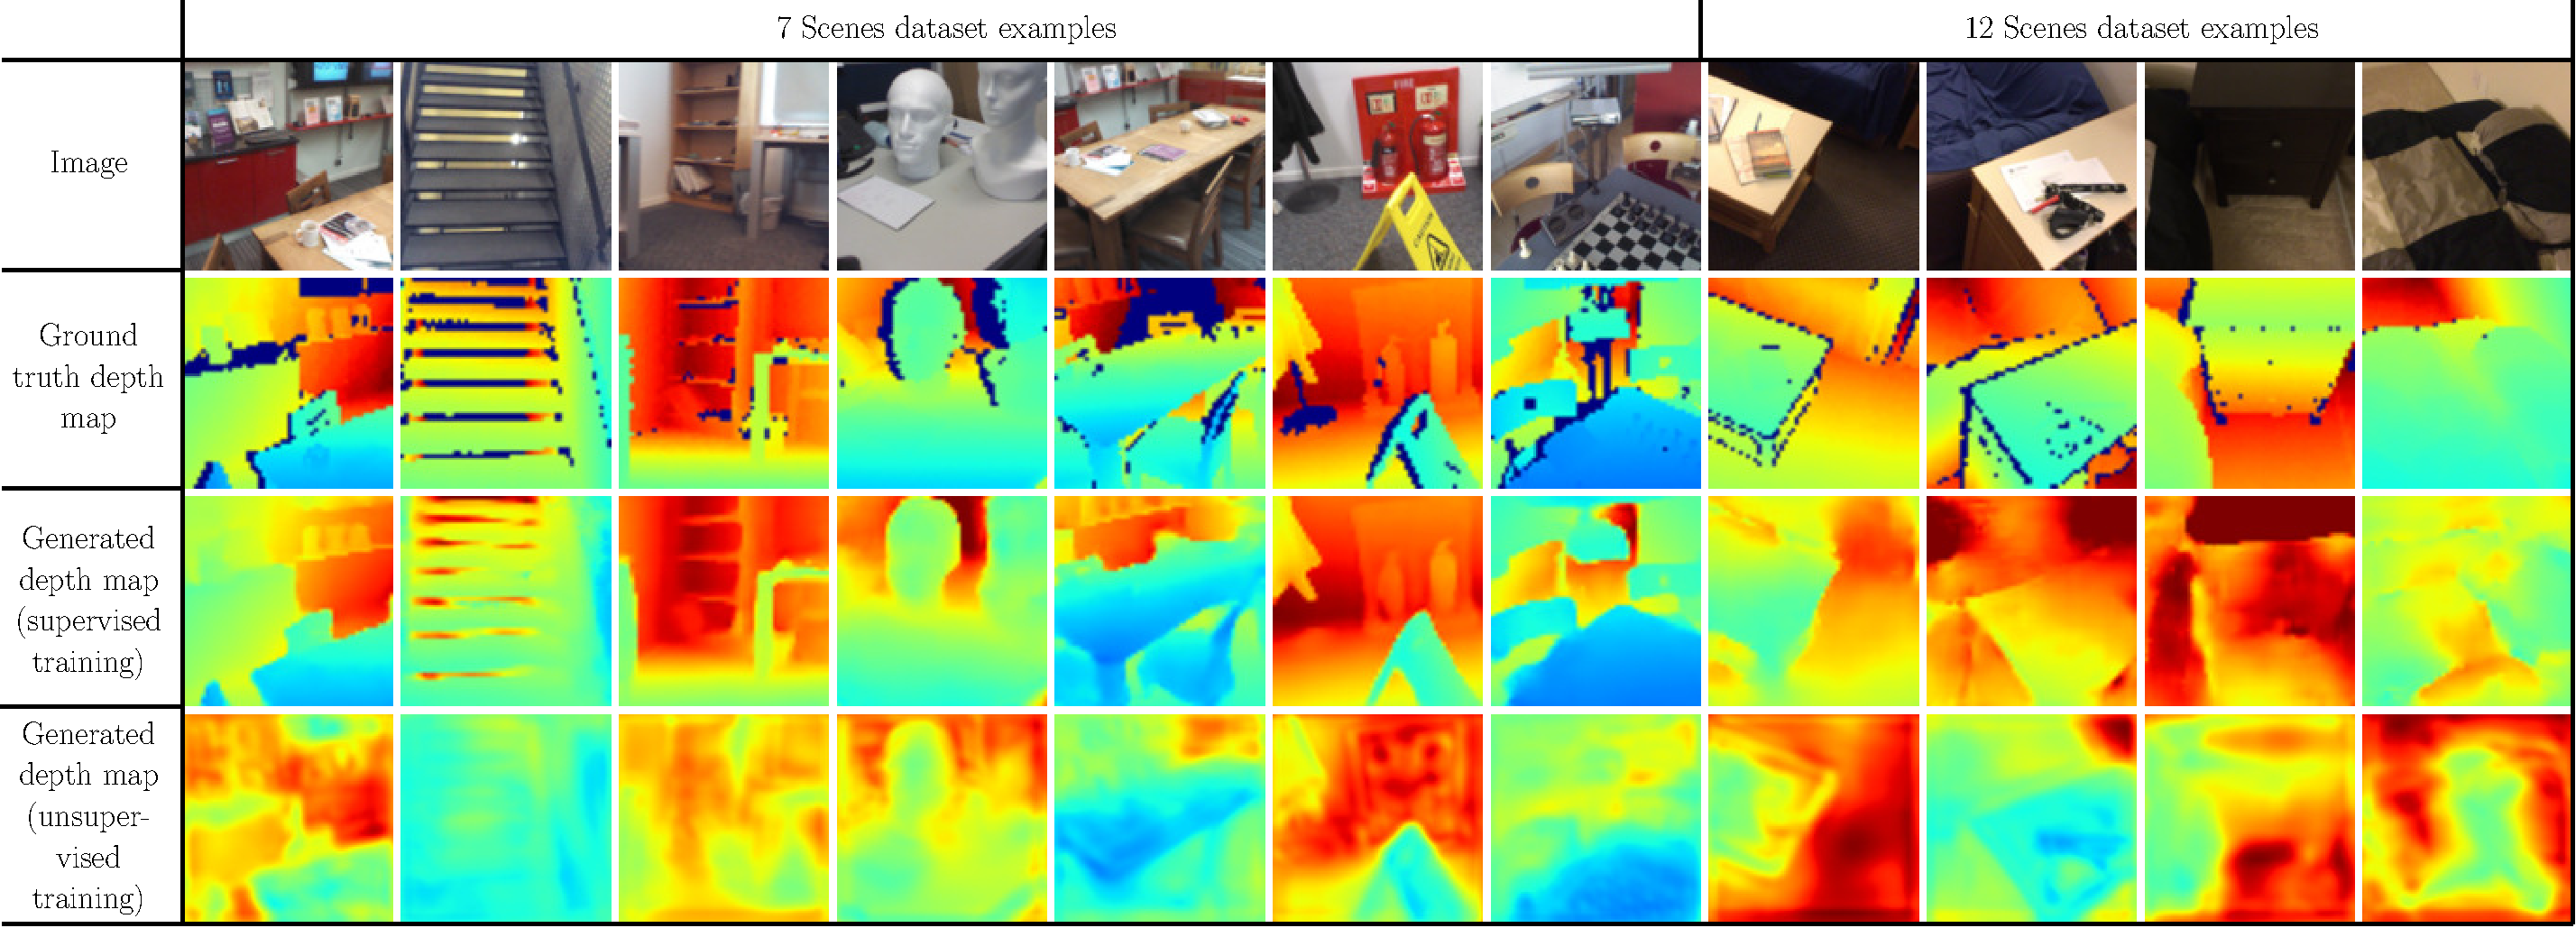
\includegraphics[width=\linewidth]{images/results/depth_map/fig1/fig1-noborder}
	\end{figure}
\end{frame}

\begin{frame}{PnlP -- Outdoor}
	\centering
	\input{tabs/pnlp/outdoor}

	\vfill	
	
	\begin{figure}
		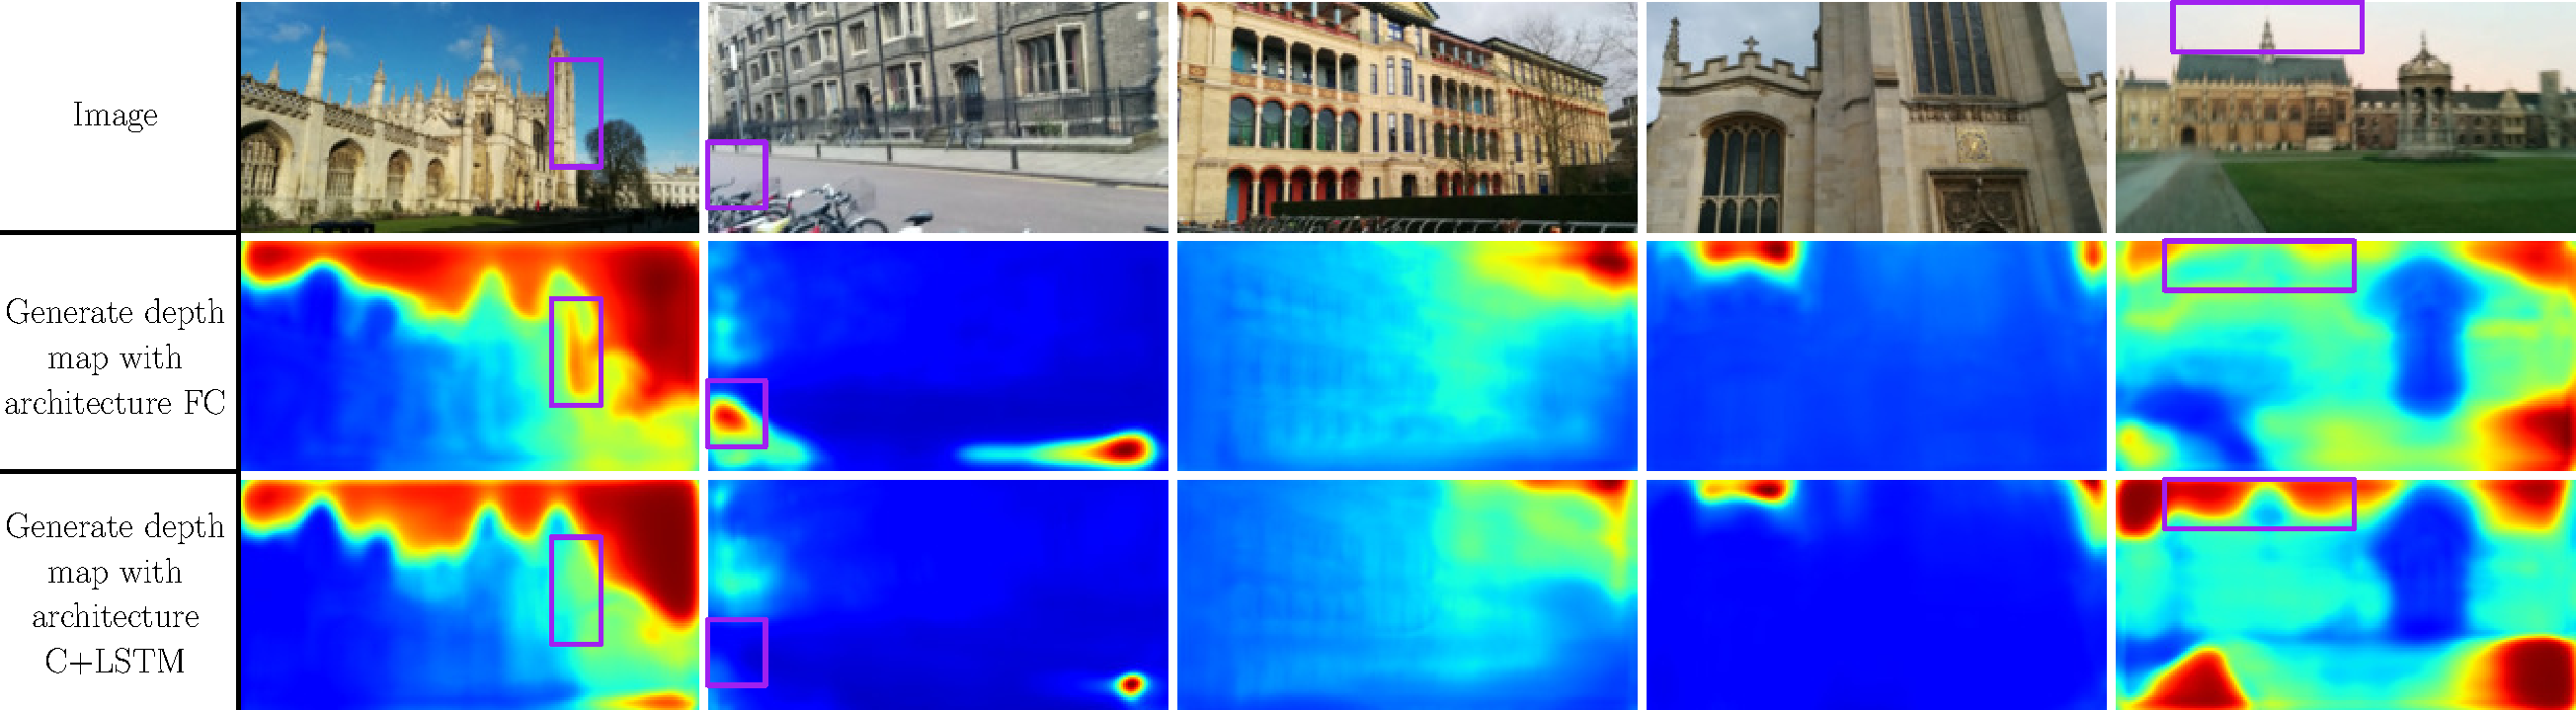
\includegraphics[width=\linewidth]{images/results/depth_map/fig2/fig2-wborder}
	\end{figure}

\end{frame}